\documentclass{tufte-handout}

%\geometry{showframe}% for debugging purposes -- displays the margins

\usepackage{amsmath}

% Set up the images/graphics package
\usepackage{graphicx}
\setkeys{Gin}{width=\linewidth,totalheight=\textheight,keepaspectratio}
\graphicspath{{graphics/}}

\title{Lipid Transport and Blood Lipid Levels}
\author{}
\date{}  % if the \date{} command is left out, the current date will be used

% The following package makes prettier tables.  We're all about the bling!
\usepackage{booktabs}

% The units package provides nice, non-stacked fractions and better spacing
% for units.
\usepackage{units}

% The fancyvrb package lets us customize the formatting of verbatim
% environments.  We use a slightly smaller font.
\usepackage{fancyvrb}
\fvset{fontsize=\normalsize}

% Small sections of multiple columns
\usepackage{multicol}

% Provides paragraphs of dummy text
\usepackage{lipsum}

% These commands are used to pretty-print LaTeX commands
\newcommand{\doccmd}[1]{\texttt{\textbackslash#1}}% command name -- adds backslash automatically
\newcommand{\docopt}[1]{\ensuremath{\langle}\textrm{\textit{#1}}\ensuremath{\rangle}}% optional command argument
\newcommand{\docarg}[1]{\textrm{\textit{#1}}}% (required) command argument
\newenvironment{docspec}{\begin{quote}\noindent}{\end{quote}}% command specification environment
\newcommand{\docenv}[1]{\textsf{#1}}% environment name
\newcommand{\docpkg}[1]{\texttt{#1}}% package name
\newcommand{\doccls}[1]{\texttt{#1}}% document class name
\newcommand{\docclsopt}[1]{\texttt{#1}}% document class option name

\begin{document}

\maketitle% this prints the handout title, author, and date

\begin{abstract}
\noindent  Lipid transport is essential to both the efficient storage, and effective use of lipids.  Due to their semi-or total insoluble nature, triglycerides, cholesterol and fatty acids present some specific technical problems in terms of transportation.  These processes rely on both carrier proteins such as albumin as well as lipoprotein particles to safely move lipids from one tissue to another.  Inefficient co-ordination of lipid transport can lead to elevated blood lipids, which are highly associated with cardiovascular disease, a major cause of death in modern society.  For more details about lipid transport refer to Chapter 18 in Lippincott's Illustrated Reviews: Biochemistry, available in reserve\cite{Ferrier2017}.
\end{abstract}

\tableofcontents

\pagebreak
\section{Learning Objectives}

\begin{itemize}
\item Explain why lipoproteins are necessary for triglyceride and cholesterol transport.
\item Describe the main carriers of cholesterol and triglyceride throughout the body, including how their apolipoproteins affect their endocytosis or catabolism.
\item Apply your knowledge of cholesterol transport to explain why someone may have changes in HDL and LDL levels.
\item Understand the etiology of high cholesterol and its potential role in atherosclerosis.  
\item Apply your understanding of cholesterol absorption, synthesis and transport to evaluate the relationships between dietary cholesterol and triglycerides and cardiovascular risk.
\item Explain the role of lipoprotein lipase in lipid transport, including how it is regulated.

\end{itemize}

\section{Key Concepts and Vocabulary}

\begin{itemize}
	\item Lipoprotein particles including:
	\begin{itemize}
		\item Chylomicrons
		\item Very Low Density Lipoproteins (VLDL)
		\item Low Density Lipoproteins (LDL)
		\item High Density Lipoproteins (HDL)
	\end{itemize}
	\item Apolipoproteins, especially ApoB40, ApoB100 and ApoCII
	\item Lipoprotein Lipase and its regulation
	\item Reverse Cholesterol Transport
	\item Trans-Intestinal Cholesterol Export (TICE)
	\item Fatty Acid Transport and Albumin
\end{itemize}

\section{Triglyceride and Fatty Acid Transport Mechanisms}

Transportation of lipids presents some logistical problems.  Since they are inherently insoluble, lipids need to be either solubilized prior to transport to other tissues via the blood stream.  This is accomplished in two ways.  One is the packaging of triglycerides and cholesterol esters into lipoprotein particles, such as the chylomicrons discussed earlier in this unit.  The second mechanism is to break triglycerides down to fatty acids, where they can bind to solubilizing proteins called albumin within the blood.

\subsection{Lipolysis and Fatty Acid Transport}

As we described in the unit about lipid oxidation, the majority of our triglyceride stores are in adipose tissue.  The release of free fatty acids and glycerol from adipose tissue is a highly regulated process, activated by adrenaline and inhibited by insulin (for more details see \citet{Zechner2012} for a review).  The transport of free fatty acids after release from adipose tissue is mediated by albumin, a very abundant protein produced by the liver.  Due to their semi-solubility, fatty acids also require transport systems and fatty acid binding proteins (abbreviated as FABP) to move through membranes and through the cytoplasm.


\subsection{Lipoprotein Particles in the Body}

In terms of moving triglycerides and cholesterol esters, we have a variety of lipoprotein particles that play different roles in the body.  These are summarized in Table \ref{tab:lipoprotein-particles}.  There are three main transport routes.  The first is from the enterocyte to the periphery, mediated by chylomicrons.  The second is from the liver to the periphery, mediated by VLDL.  The third is from the periphery back to the liver, mediated by HDL and LDL.  We will discuss each of these in the next few sections.

\begin{margintable}
\centering
\caption{Summary of lipoprotein particles.}
\label{tab:lipoprotein-particles}
\begin{tabular}{@{}ccc@{}}
\toprule
\textbf{Particle} & \textbf{Source} & \textbf{Destination}       \\ \midrule
Chylomicron       & Enterocyte      & Adipose, Muscle, Liver \\
VLDL              & Liver           & Adipose, Muscle            \\
IDL               & VLDL          & Liver or LDL \\
HDL               & Endothelial     & LDL                        \\
LDL               & IDL/HDL             & Liver                      \\ \bottomrule
\end{tabular}
\end{margintable}


The goal of these lipoprotein particles is to move lipids from the source\sidenote{The source of chylomicrons transporting dietary lipids is the enterocyte, or the source of VLDL is the liver; the function of lipoproteins is to trasnport the lipids from both these sources, enterocyte and liver} to peripheral tissues which might be better equipped to utilize or store these lipids.  As summarized in Table \ref{tab:apolipoproteins}, these particles are characterized by distinct lipoproteins.

\begin{margintable}
\centering
\caption{Apolipoprotein summary.  Some key things to remember, ApoB48 is specifically made in the enterocyte.  ApoB100 and ApoE are the ligands for the LDL Receptor allowing for LDL uptake in tissues expressing the LDL receptor (mainly the liver).  ApoCII is a coenzyme for LPL thus activating it and allowing for lipid extraction to peripheral tissues.}
\label{tab:apolipoproteins}
\begin{tabular}{@{}cllcc@{}}
\toprule
\textbf{Particle} & \textbf{ApoA} & \textbf{ApoB} & \textbf{ApoC} & \textbf{ApoE} \\ \midrule
Chylomicron       &  AV         & B48           & CII/CIII           & E             \\
VLDL              &   AV            & B100          & CI/CII        & E             \\
IDL               &                  & B100         &        &   E \\
HDL               & AI/AII          & B100          &               &             E  \\
LDL               &         & B100          &               &              
\end{tabular}
\end{margintable}
\section{The Role of Chylomicrons and VLDL}

Both chylomicrons and VLDL function to move lipids to peripheral tissues, either from the gastrointestinal tract or the liver, respectively.  These particles transport primarily \emph{neutral lipids} rather than free fatty acids.  Their assembly is dependent on the production of the apolipoproteins and the presence of phospholipids, especially phosphatidylcholine that is important for their synthesis.   If choline levels are limited, either due to less active variants in \textit{PEMT} or reduced choline dietary intake, the liver will be less able to assemble VLDL.  This can result in increased hepatic steatosis, potentially leading to non-alcoholic fatty liver disease.

\subsection{The Role and Regulation of Lipoprotein Lipase}

Both VLDL and chylomicrons are targeted to peripheral tissues.  This specificity is mediated by Apolipoprotein CII.  This lipid acts as an activator of a triglyceride lipase known as \emph{Lipoprotein Lipase} or LPL.  This lipase resides on the lumen of blood vessels, adjacent to muscle and adipose tissues.  Once activated by ApoCII binding, LPL breaks down the triglycerides in the particle and releases its free fatty acid content.  These free fatty acids enter the cell where they can be stored (if they enter into the adipocytes), or are used as fuel (if they enter into the muscle cells).  The levels of LPL are inversely regulated in adipose and muscle tissue. For example, insulin promotes LPL transcription in adipose tissue\sidenote{To promote lipid storage.  This is accomplished by both transcriptional and post-translational mechanisms, reviewed in \citet{Kersten2014}.} but decreases LPL transcription in muscle \citep{Spooners1979}.  The inverse is true during fasting, where the muscle LPL trasncription is increased while that of the adipose tissue is reduced thus promoting muscle uptake of fat to be used as energy, while limiting adipose tissue ability to store this fat in times of energy need (fasting). 

\newthought{LPL is inactivated by diets high in saturated fats.}  This means that when saturated fat levels are increased, LPL activity is reduced. You can imagine how this is unbeneficial to the body, as the lipids in the blood cannot be taken up into the muscles or adipose tissue, therefore remaining in the blood and circulation.  This is a negative feedback mechanism wherein intracellular lipids can signal to the LPL on the extracellular surface to prevent additional fat uptake (see Figure \ref{fig:angptl4}).  The molecular underpinnings of this phenomena have recently been determined and involve the transcriptional activation of a protein called ANGPTL4\sidenote{Unhelpfully, an abbreviation for Angiopoietin-like 4.}.  ANGPTL4 is induced when excess fatty acid levels in the cell activate the transcription factor PPAR$\alpha$.  ANGPTL4 is then secreted where it binds to and inhibits the activity of LPL (more details about this can be found in the recent review by \citet{Dijk2014}).  Mutations in either the \textit{LPL} or \textit{ANGPTL4} genes result in either impaired, or enhanced blood lipid clearance, respectively and as a result either lead to an increased or decreased risk of cardiovascular disease \citep{Article2016b}.

\begin{marginfigure}
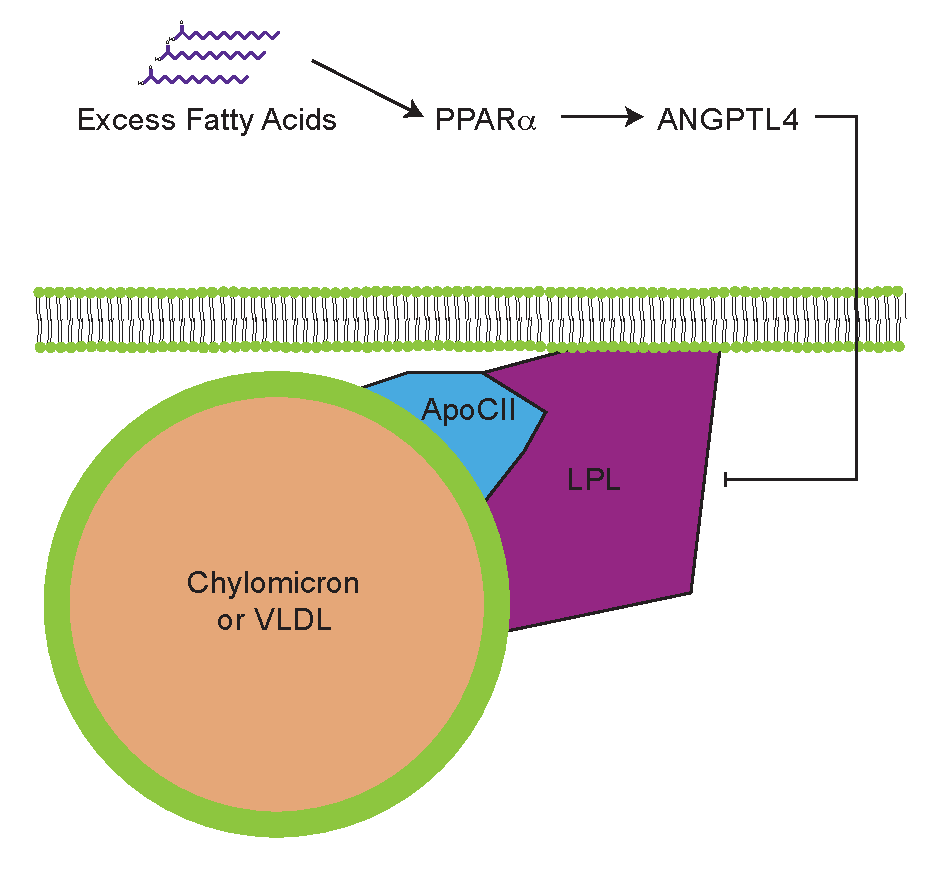
\includegraphics{figures/Angptl4-PPARa.pdf}
\caption{Regulation of Lipoprotein Lipase (LPL) by ANGPTL4.}
\label{fig:angptl4}
\end{marginfigure}

\newthought{Depleted VLDL are known as IDL, whereas depleted chylomicrons are known as chylomicron remnants.}  Once these lipoproteins have delivered their triglyceride content into cells, they are either known as chylomicron remnants or intermediate\sidenote{This indicates that this lipoprotein has intermediate density that falls in between VLDL and LDL's density} density lipoproteins (IDL).  Due to the presence of ApoE on their surface, chylomicron remnants and IDL particles can be absorbed by the liver where the apolipoproteins and phospholipids can be reused.

\newthought{\textit{APOE} variants are associated with disease risk}  since this apolipoprotein is present on both chylomicrons and VLDL that then form IDL .  There are four variants of the \textit{APOE} gene numbered 1-4\sidenote{These are variants of the same gene, not different genes}.  Of these isoforms, ApoE2 is thought to be protective while ApoE4 is considered a risk factor for late-onset Alzheimer's disease \citep{Poirier1993,Corder1993}.  

\section{Reverse Cholesterol Transport}

Cholesterol is primarily disposed of via bile salt generation and excretion, a process that starts in the liver.  Therefore cholesterol, which is made throughout the body, is primarily trafficked to the liver, a process known as \emph{Reverse Cholesterol Transport}.  This process is mediated by both HDL and LDL particles.  To separate blood lipids between reverse and forward transport processes, sometimes the ratio betwen ApoB and ApoAI is determined\sidenote{Consider based on the data in Table \ref{tab:apolipoproteins} what this ratio is actually measuring.  As a hint, a high ApoB100/ApoA1 ratio is indicitave of elevated cardiovascular risk.}.  An alternate cholesterol disposal pathway is through the intestine, a process known as trans-intestinal cholesterol excretion\sidenote{TICE}.  In this pathway, cholesterol is transported by either HDL or LDL directly to the intestine for efflux.  Estimates vary, but we think that somewhere between 20 and 40\% of cholesterol excretion is through TICE, with the remainder being through biliary transport \citep{Temel2015}.

\subsection{Synthesis and Role of HDL}

High density lipoprotein particles start off as nascent particles containing ApoAI, ApoAII and very little cholesterol.  As they pass through the circulation, they bind cholesterol from the plasma membrane of tissues and become enriched with cholesterol.  Since most tissues make but cannot dispose of cholesterol, HDL is important for scavenging excess cholesterol from our cells. The HDL particles may be endocytosed in the liver where cholesterol can be disposed, but most often they transfer their cholesterol to LDL particles using an enzyme known as cholesterylester transfer protein\sidenote{Abbreviated as CETP}.  This ensures that triglycerides are packaged in the LPL-accessible particles for peripheral transport to be used by peripheral tissues, while excess cholesterol is delivered back to the liver or intestine for excretion.   Inhibition of CETP results in an increase in the amount of  HDL cholesterol in the blood and thus CEPT inhibition was a heavily invested pharmacological area, but these drugs have shown limited cardiovascular benefits.  The current thinking in this area is that high HDL cholesterol is a marker of lowered cardiovascular risk but does not cause lowered cardiovascular risk by itself.

\subsection{LDL-mediated Transport to the Liver}

Low density lipoproteins are generated when IDL derived from VLDL remains in the circulation, or when cholesterol is passed from an HDL to an IDL particle.  These particles tend to be cholesterol rich, since the triglycerides have been already taken up due to the actions of LPL at peripheral tissues.  These particles would normally be endocytosed by the liver where LDL receptors are found.  LDLR levels are under control of the SREBP2.  Recall that when intrahepatic cholesterol levels are high, SREBP2 is inactive, and thus LDLR would not be produced.  This means that when the liver has sufficient cholesterol, LDL particles remain in the circulation\sidenote{As a thought exercise, consider what would happen if you had a \textit{LDLR} mutation, how would that affect cholesterol retrieval?  How do you think it would affect cholesterol synthesis?  This is the case for individuals with a disease known as familial hypercholesterolemia.}.  LDL cholesterol levels are correlated with coronary events.  If one wants to understand the levels of LDL cholesterol in a person there are two measures to consider.  By looking at how much cholesterol is in the LDL fraction (LDL-C, should be less than 100 mg/dL) or how many LDL particles are present in the blood.  Since each LDL contains one, and only one ApoB100 particle, and since LDL particles vastly outnumber VLDL particles, then if you determine the concentration of ApoB100 in blood, then that is a measure of LDL particle number.  Recent studies have suggested that it is this particle number, more so than the amount of cholesterol in the LDL fraction, that is more predictive of cardiovascular events, though generally both the cholesterol content in LDL and the LDL particle number incresae for most people simultaneously \citep{Cromwell2007,Mora2007}.

\subsection{Cholesterol Export to Bile}

Within the liver, bile salt synthesis is controlled by the activity of 7-$\alpha$-hydroxylase\sidenote{We discussed this in the lipid digestion lecture} and exported to the gallbladder for release into the digestive system.  Separate from the SREBP2-dependent cholesterol regulatory system, the production of bile salts is sensed by the FXR sensing system\sidenote{FXR is a bile acid sensor expressed in entero-hepatic tissues.}.

\section{Blood Lipids and Cardiovascular Risk}

If lipid transport systems (of VLDL and LDL) have exceeded their ability to store lipids, then VLDL and LDL lipids remain in the blood.  Akin to the hyperglycemia associated with impaired glucose disposal, and excessive glucose production, hyperlipidemia is associated with cardiovascular disease due to impaired lipid disposal.  Since triglycerides can be metabolized into energy by most tissues, but cholesterol cannot, hypercholesterolemia in particular has been long associated with cardiovascular risk \citep{Keys1963}.

Since cholesterol may exist in several lipoprotein particles, a more prognostic indicator of cardiovascular risk is the amount of cholesterol in HDL particles relative to the amount of cholesterol in LDL particles, with the latter being more pathogenic\sidenote{HDL cholesterol levels may indicate a surplus of cholesterol transport particles, whereas LDL cholesterol likely indicates a surplus of cholesterol that cannot be absorbed by the liver.}.  Several mechanisms for LDL's specific association with cardiovascular risk have been proposed, but one possibility is that excess LDL is absorbed in blood vessel walls, promoting both atherosclerosis\sidenote{The lipid-based coating of arteries, causing arteries to become narrower and reducing their vascular flexibility.} and increasing the risk of thrombosis\sidenote{The release of a blood clot, often by lysis and release of an atherosclerotic plaque.  This blood clot could travel to the brain or heart where a stroke or heart attack may occur.}.

\newthought{From a dietary standpoint}, data from several US-based cohort studies demonstrated that diets lower in saturated fat intake are positively associated with both total and LDL cholesterol, and therefore associated with reductions in cardiovascular disease \citep{Anderson1987,Wang2016b}.  This has recently been challenged by a large-multi country study\sidenote{This is known as the PURE study, which evaluated over 135 000 participants in 18 countries.} which indicated that increased carbohydrate intake plays a key role, maybe more so than saturated fats with respect to cardiovascular disease \citep{Dehghan2017}.  For this large multi-ethnic study, there is some debate about whether regional dietary differences are fully accounted for, or if this is more reflective of diet-disease risk in a more diverse dataset.  In either case, both studies agree that more LDL cholesterol is generally associated with increased heart disease risk.

\bibliography{library}
\bibliographystyle{plainnat}

\end{document}
